\section{Binární halda}\label{sec:halda}

Uveďme motivační příklad na úvod. Mějme seznam čísel, z něhož chceme (pokud možno co nejrychleji) vybrat minimální/maximální hodnotu. Pro maximum bychom sestavit následující jednoduchý algoritmus.
\begin{pseudo}{Max}[Seznam čísel $x_1,x_2,\dots,x_n$][Maximální hodnota seznamu \textit{m}]
    $m\gets x_1$\\
    \begin{For}{$i=1,2,\dots,n$}
        \begin{If}{$x_i>m$}
            $m\gets x_i$
        \end{If}
    \end{For}
\end{pseudo}

Časová složitost bude zjevně $\bigO{n}$, neboť algoritmus prochází všech $n$ prvků. Takovou úlohu lze však řešit rychleji, pokud si prvky vhodně uspořádáme. K tomu můžeme použít tzv. \emph{haldu}. 
\begin{definition}[Minimová binární halda]\label{def:binarni_halda}
    Minimová binární halda je datová struktura tvaru binárního stromu, kde v každém vrcholu je uložena \emph{právě jedna} hodnota (tzv. \emph{klíč}, pro vrchol $v$ budeme značit jeho klíč $k(v)$) a navíc platí:
    \begin{enumerate}[label=(\roman*)]
        \item\label{binhalda_podminka_1} každá hladina je plně obsazena, kromě poslední
        \item\label{binhalda_podminka_2} a je-li $v$ libovolný vrchol a $s$ jeho syn, pak $k(v)\leqslant k(s)$.
    \end{enumerate}
\end{definition}

\begin{figure}[h]
    \centering
    \begin{subfigure}{6cm}
        \centering
        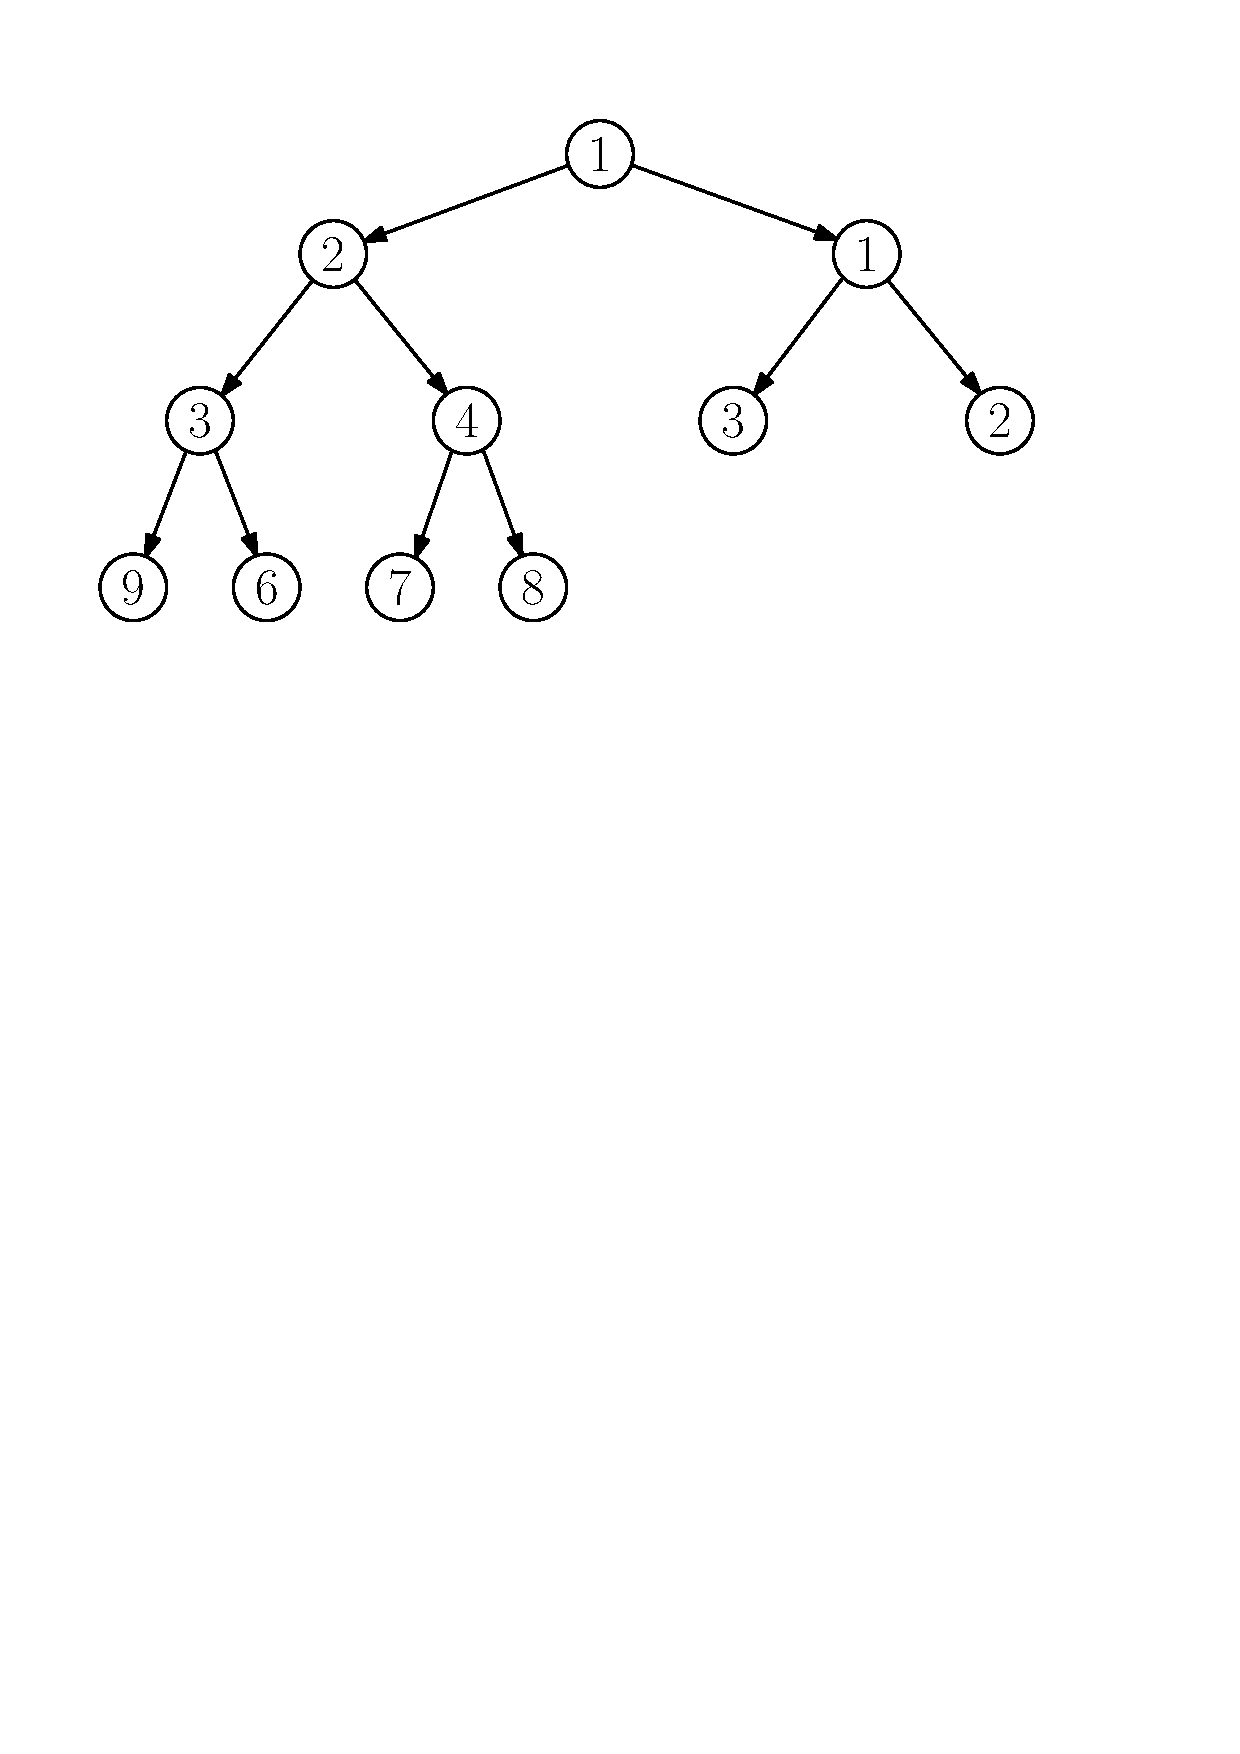
\includegraphics[scale=.4]{ch01_halda}
        \caption{Korektní halda.}
        \label{subfig:korektni_halda}
    \end{subfigure}
    \quad
    \begin{subfigure}{5cm}
        \centering
        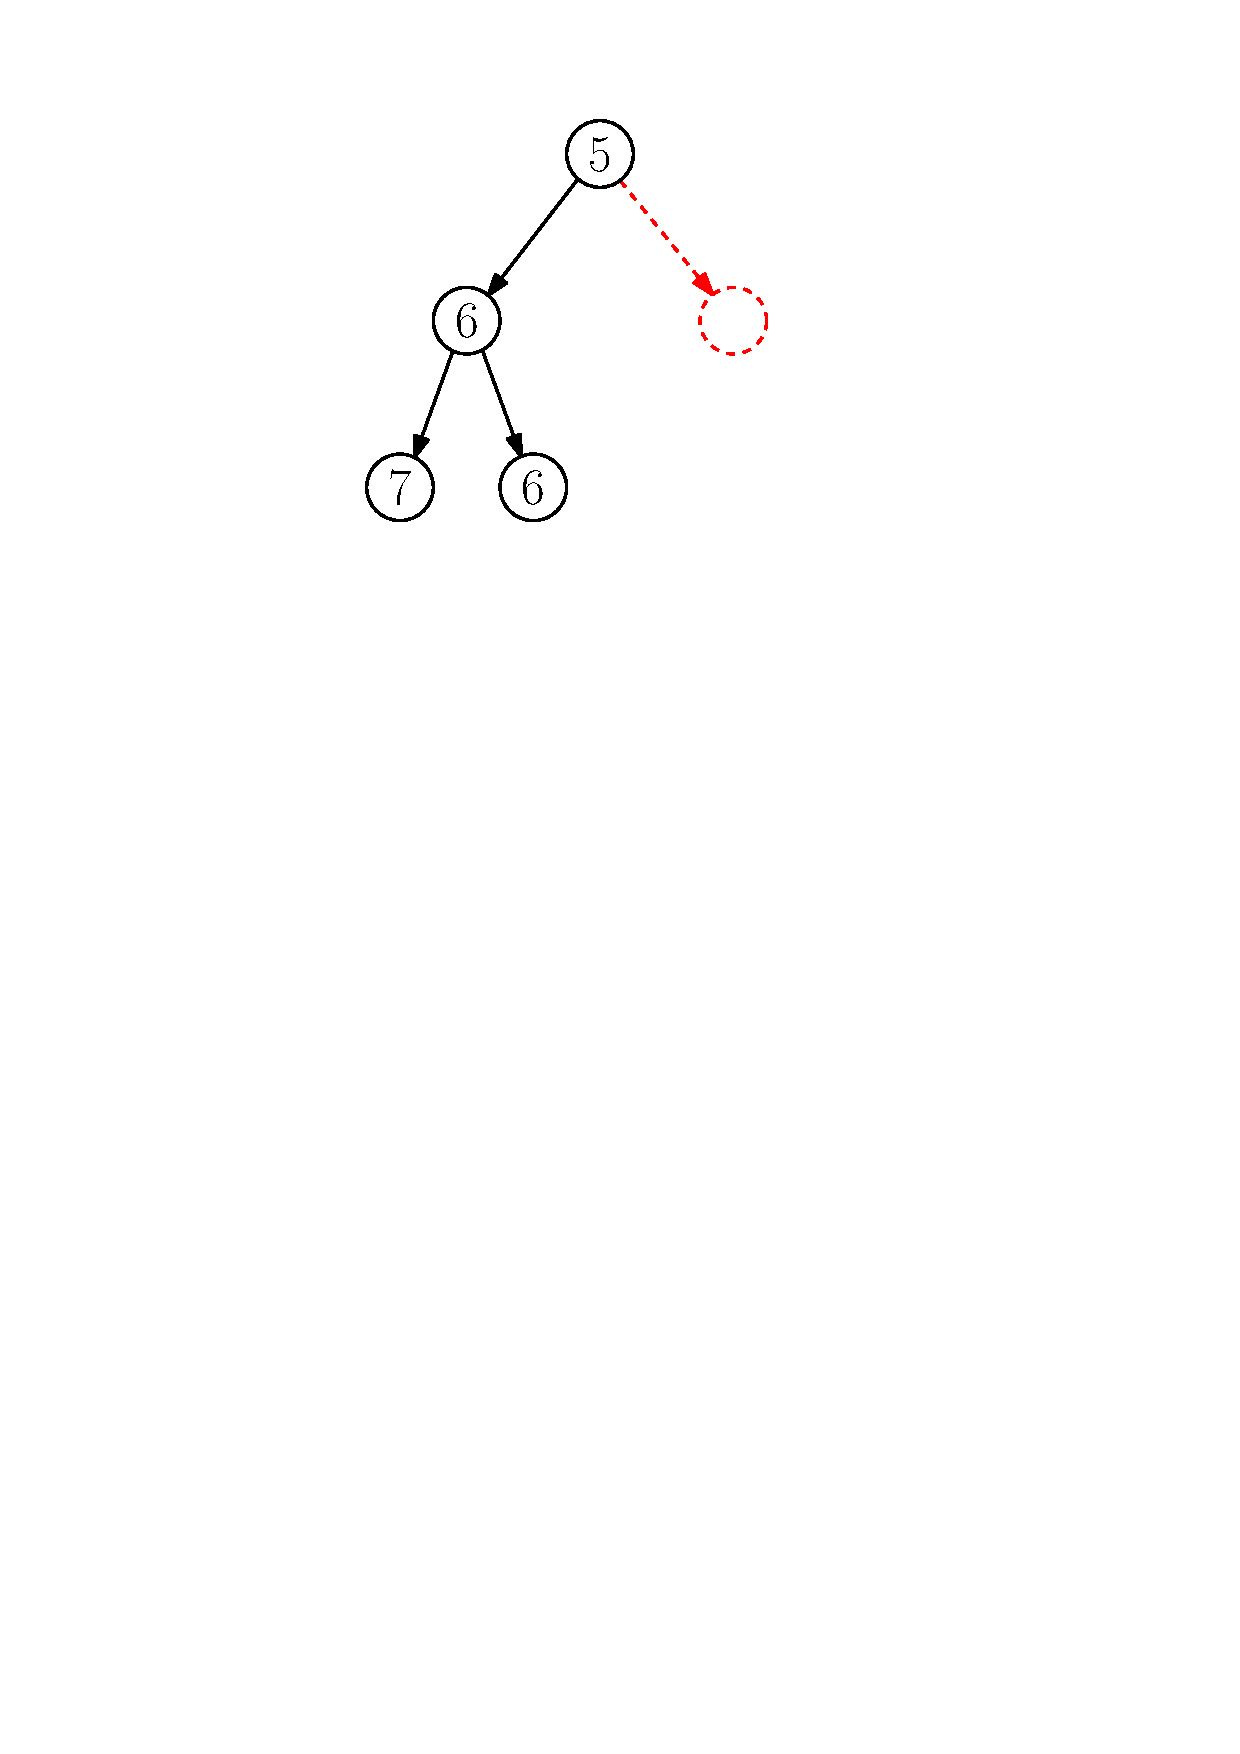
\includegraphics[scale=.4]{ch01_nekor_halda_1}
        \caption{Chybějící vrchol v 1. hladině.}
        \label{subfig:nekorektni_halda_1}
    \end{subfigure}
    \quad
    \begin{subfigure}{5cm}
        \centering
        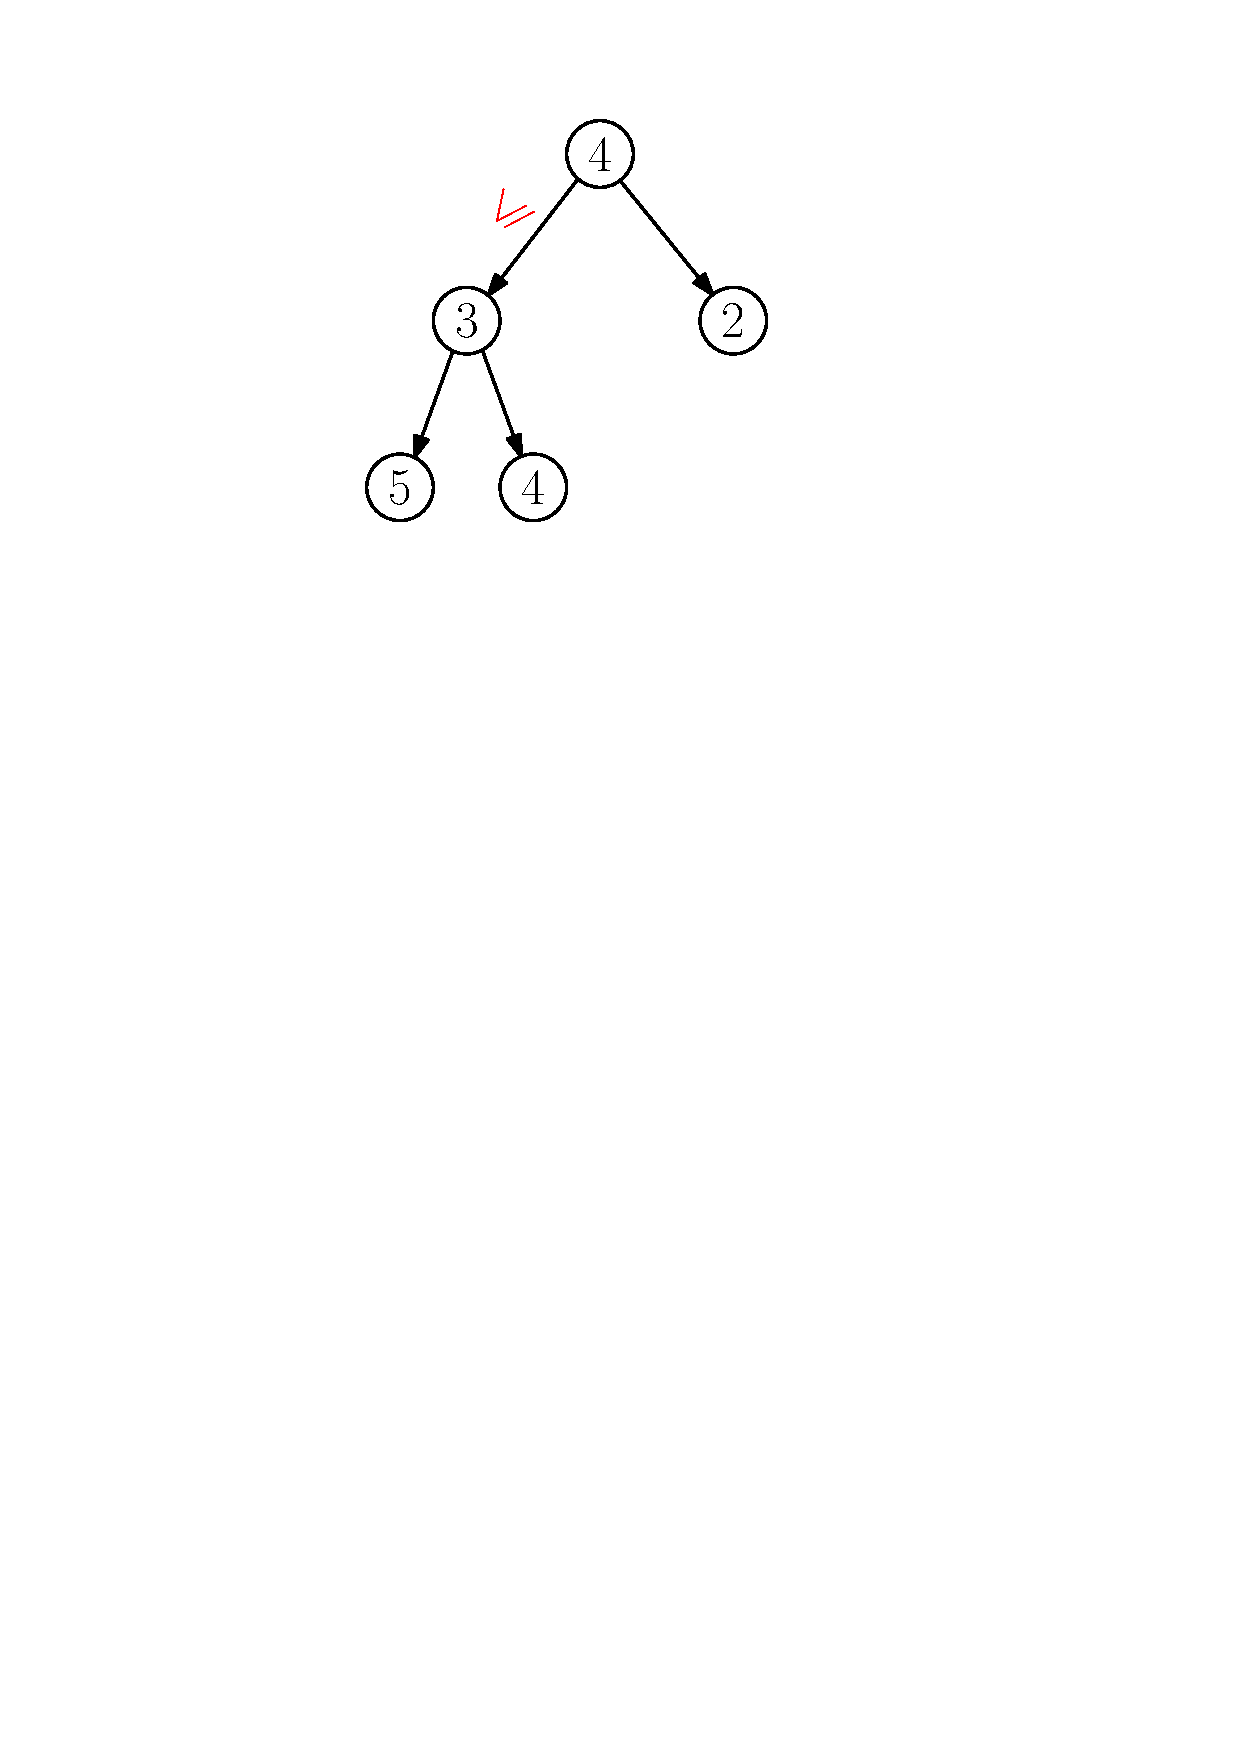
\includegraphics[scale=.4]{ch01_nekor_halda_2}
        \caption{Klíč levého syna je menší než klíč kořene.}
        \label{subfig:nekorektni_halda_2}
    \end{subfigure}
    \caption{Příklady korektních a nekorektních hald.}
    \label{fig:halda_modely}
\end{figure}

Zde se nyní na chvíli pozastavme. Podmínka \ref{binhalda_podminka_2} v definici binární haldy \ref{def:binarni_halda} má za následek totiž velmi příjemnou vlastnost, když se podíváme, kde se v haldě nachází minimum. Pokud se budeme pohybovat od kořene směrem "dolů", hodnoty ve vrcholech se budou pouze zvětšovat, neboť klíče synů mají musí mít vždy stejnou nebo větší hodnotu než klíč v rodiči. Minimum se tak vždy nachází \emph{v kořeni stromu}, což znamená, že zjistění minima tak můžeme provést v \emph{konstantním čase} $\bigO{1}$.
\notebox{Pokud bychom chtěli maximovou binární haldu, bude definice \ref{def:binarni_halda} vypadat obdobně, akorát v podmínce \ref{binhalda_podminka_2} bude obrácená nerovnost, tj. $k(v)\geqslant k(s)$ (klíč v rodiči má vždy stejnou nebo vyšší hodnotu než klíče v jeho synech). Maximum se bude opět nacházet v kořeni haldy.}